\section{Using \smyrna} \label{sec:using}

One starts \smyrna\ as with any program, either using a command interpreter to
execute it or double-clicking on its icon. From the command line, 
it accepts a single argument giving the
file name of a graph to be viewed.

This will open a main window for \smyrna\ similar to 
that shown in Figure~\ref{fig:main0}.
\begin{figure}[ht] 
\begin{center}
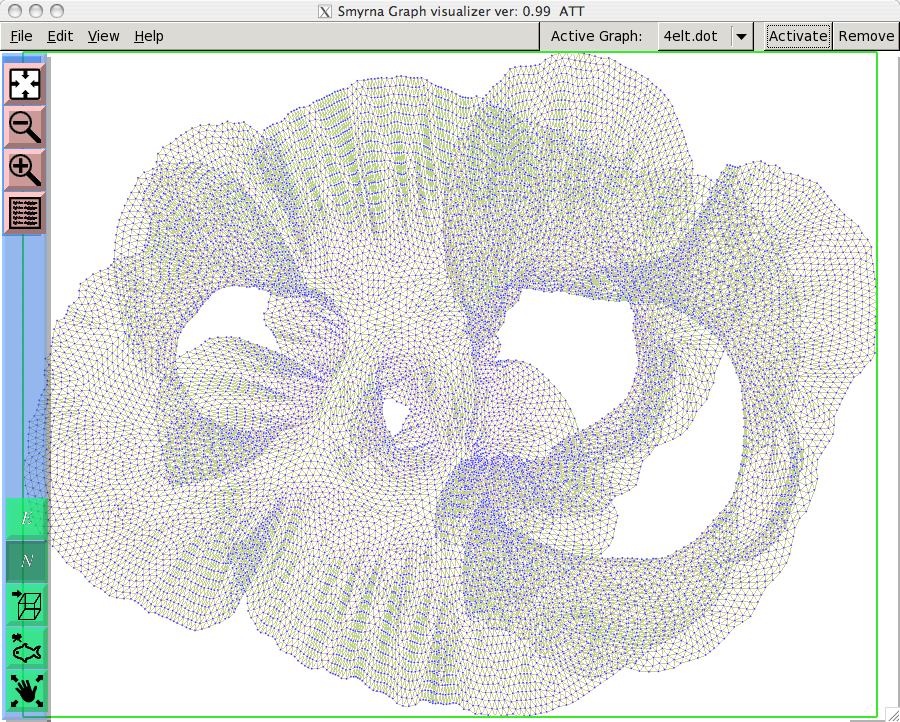
\includegraphics[scale=.3]{figures/smyrna.png}
\caption{\small Typical \smyrna\ view.}
\label{fig:main0} 
\end{center}
\end{figure}
The window has a fairly typical layout. There is a menu bar across the top,
with some additional widgets on the right side of it. There is a control bar
of buttons down the left side. The remainder of the window is the display area.

\subsection{Opening a graph}
If no file name is given on the command line, one can use 
{\tt File->Open} to open a graph file. This can also be used
read in additional graphs. When a new graph is read in, it is made
the {\it active} graph, and the previous graph is added to the
list of open graphs. One can make an open graph the new active
graph by using the {\tt Active Graph} menu at the top right
of the main window, picking the desired
graph, and then clicking on the {\tt Activate} button.

Being able to switch back and forth between open graphs can be
useful when analyzing graphs. However, due to resource consumption,
one should avoid having too many open graphs. You can close a
graph the same way that you activate it, except clicking on the
{\tt Remove} button rather than {\tt Activate}. 

\subsection{Navigation}
To zoom in and out on a graph, you use the scroll wheel or ball
on the mouse. Or you can use the plus and minus magnifying glasses

\includegraphics{figures/zoomin.png} 
\includegraphics{figures/zoomout.png}
on the left-hand icon bar.

To pan, click and hold down the left mouse button, and move the
mouse. Releasing the mouse stops the panning.

Sometimes during navigation, you may find yourself in some obscure corner
of the graph, or you've lost the graph entirely. By clicking on the top
button

\includegraphics{figures/center.png}
on the left icon bar, the view is reset so that the graph is 
centered in the window, and just large enough
to fill it. 

\subsection{Selection}
{\it Smyrna} has a notion of selected nodes and edges. 
To pick a single node or edge, right click on it. The color will
change to indicate the selection; in addition, an
attribute of the object may be displayed. You can use the Labels
tab (Section~\ref{subsubsec:labels}) to specify which attribute you wish to see.
If right clicked a second time, the object is unselected.
Multiple objects can be selected.

One can also select multiple items by holding down the right mouse
button and sweeping out a region. One can do this multiple times;
the selected set is the union of all selections.
What is selected is determined by the E and N buttons on the control bar, which
activate the selection of edges and nodes respectively. Initially, only nodes
can be selected.
\begin{comment}
\bf Can one unselect multiple nodes, but not all?
\end{comment}

The button

\includegraphics{figures/pan.png}
at the bottom of the control bar can be used to unselect everything.
\begin{comment}
Do we still want cluster selection? What does that do?
Should one be able to unselect by sweeping?
\end{comment}

Choosing {\tt Edit->Node List} opens the Node List widget (Section~\ref{sec:nodelist}),
which provides a text view of the selected nodes. It also provides the opportunity
to save the selected nodes as a subgraph.

\subsection{3D in \smyrna}
\label{sec:3D}
To move from a 2D to a 3D view, click the button 
\includegraphics{figures/3D.png}
found in the control bar. Pan and zoom are achieved the same way they are in 2D.
For rotation in 3D, hold down the left shift key, then click and hold 
down the left mouse button, and move the mouse.
Returning back to 2D is done by clicking the control bar button

\includegraphics{figures/2D.png}.

\subsection{Graphical Node and Edge Attributes}
To display more information about the graph, especially attributes
that may be associated with nodes or edges, one can use various
display attributes. The principal such attribute is color, stored
as the {\tt color} attribute in a node or edge. The attribute can
be set already when the graph is read in, or it can be attached
using the Attribute tab or the Script tab of Settings widget.
If the color is not explicitly set, \smyrna\ provides default values
which can be set using the General tab of the Settings widget.

For cluttered drawings, it can sometimes help to play down parts of the graph.
\smyrna\ allows you turn off the drawing of either nodes are edges. There 
are check boxes for this also on the General tab.
You can also reach a middle ground by having the edges or nodes drawn, but making
them more transparent. To do this, one uses the Node Alpha and Edge Alpha sliders
on the Graph tab.

The Graph tab also provides a Node Size slider. With this, you can uniformly
increase or decrease the size of the nodes. If Node Shape is set to Spherical,
you can set the size attribute of nodes to get a variation in node sizes. 
The attribute is used as a scale factor, so a size less than 1 will cause a node
to shrink relative to other nodes while a size greater than 1 will enlarge the node.

For large graphs, lack of screen space means you usually want to see nodes drawn as small disks.
This holds if Node Shape is set to either OpenGL dots or Spherical. The former is quicker to draw,
but at present does not allow varying sizes among nodes. (The Custom shape is not implemented.)
For smaller graphs with xdot attributes attached, \smyrna\ will use the xdot information to
draw the nodes and edges.  

\subsubsection {Defining and setting attributes}
Attributes can be defined and set in \smyrna\ using either the Attributes tab or \gvpr\ via the
Script tab. For setting atttributes, the former works on the set of selected nodes. 

\subsection{General Graph Manipulation}
\label{sec:gvpr}
There are controls in \smyrna\ for the most common operations such as navigation, selection
by mouse and simple attribute queries. For more complex selection criteria, and general
analysis and manipulation of graphs, \smyrna\ is integrated with the \gvpr\ graph processor. 
The main interface to \gvpr\ is provided by the Script tab (Section~\ref{sec:gvprtab}), though
\smyrna\ also uses \gvpr\ for various internal operations.

To use \gvpr, you write a script in the \gvpr\ language, which is then applied against an input 
graph. With the language, you can specify operations to be performed when the graph is first scanned;
operations to be performed when each node or edge is visited; and operations to be performed after
all node and edge processing has been done. Node and edge statements can have a boolean guard; with
this, the action is only performed if the guard is true.
As a simple example, the script
\begin{verbatim}
N[color=="blue"]{selected="1"}
\end{verbatim}
causes \gvpr\ to mark all blue nodes as selected.

Though \gvpr\ is primarily designed for working with graphs, it incorporates the C language
expression model, and provides many general-purpose C-like functions such as {\tt printf} and file I/O,
string manipulation functions, and associative arrays. A more complete discussion of the use of
\gvpr\ is outside of the scope of this document. The reader is referred to the \gvpr\ man page for
further information. 

\subsection{Topological Fisheye Views}
\label{sec:topfish}
